% \iffalse
\let\negmedspace\undefined
\let\negthickspace\undefined
\documentclass[journal,12pt,twocolumn]{IEEEtran}
\usepackage{cite}
\usepackage{amsmath,amssymb,amsfonts,amsthm}
\usepackage{algorithmic}
\usepackage{graphicx}
\usepackage{textcomp}
\usepackage{xcolor}
\usepackage{txfonts}
\usepackage{listings}
\usepackage{enumitem}
\usepackage{mathtools}
\usepackage{gensymb}
\usepackage{comment}
\usepackage[breaklinks=true]{hyperref}
\usepackage{tkz-euclide} 
\usepackage{listings}
\usepackage{gvv}                                        
\def\inputGnumericTable{}                                 
\usepackage[latin1]{inputenc}                                
\usepackage{color}                                            
\usepackage{array}                                            
\usepackage{longtable}                                       
\usepackage{calc}                                             
\usepackage{multirow}                                         
\usepackage{hhline}                                           
\usepackage{ifthen}                                           
\usepackage{lscape}
\usepackage{placeins}
\usepackage{xparse}


\newtheorem{theorem}{Theorem}[section]
\newtheorem{problem}{Problem}
\newtheorem{proposition}{Proposition}[section]
\newtheorem{lemma}{Lemma}[section]
\newtheorem{corollary}[theorem]{Corollary}
\newtheorem{example}{Example}[section]
\newtheorem{definition}[problem]{Definition}
\newcommand{\BEQA}{\begin{eqnarray}}
\newcommand{\EEQA}{\end{eqnarray}}
\newcommand{\define}{\stackrel{\triangle}{=}}
\theoremstyle{remark}
\newtheorem{rem}{Remark}

\graphicspath{ {./figs/} } 

\begin{document}

\bibliographystyle{IEEEtran}
\vspace{3cm}

\Large\title{NCERT Question 10.5.2.5}
\large\author{EE23BTECH11032 - Kaustubh Parag Khachane $^{*}$% <-this % stops a space
}
\maketitle
\newpage
\bigskip

\renewcommand{\thefigure}{\theenumi}
\renewcommand{\thetable}{\theenumi}
\large\textbf{Question 10.5.2.5} : \normalsize Find the number of terms in each of the following APs. Then express each term as x(n) and find the z transform and its ROC: 

\brak{i} 7, 13, 19, ... 205

\brak{ii} 18, 15$\frac{1}{2}$, 13, ... -47

\vspace{4mm} 

\large\textbf{Solution} :\normalsize
\vspace{4mm}
\begin{table}[!ht] 
\centering
\setlength{\extrarowheight}{8pt}
\begin{tabular}{|l|l|l|}
    \hline
    \textbf{Parameter} & \textbf{Description} & \textbf{Value} \\
    \hline
     m & Mass of object & 10 Kg \\\hline
     $\mu$ & Frictional coefficient \brak{static} & 0.25\\\hline
     x\brak{t} & Displacement of block &  \\\hline
     $x\brak{0}$ & Initial displacement & 0 \brak{assumed} \\\hline
     g & Gravitational acceleration & 10 $m/s^2$ \\\hline
     $F_s$ & Spring force &  \\\hline
     f & frictional force &  $\mu$ N \\\hline
     N & Normal Force & mg $cos\brak{\theta}$ \\\hline
    \end{tabular}
  \vspace{4mm}
 \caption{Parameter Table}
 \label{tab:table0_xe80}
\end{table}

\textbf{\brak i} 

$x_{1}\brak{n} = x_{1}\brak{0} + nd_{1}$

If 205 is the $n{th}$ term of the series, we have :
\begin{align}
&205 = 7 + \brak{n}6\\ 
\implies&  198 = 6n\\
\implies&  33 = n
\end{align}
$\therefore$ There are 34 elements in the series.

\vspace{4mm}

\textbf{\brak{ii}} 

$x_{2}\brak{0} = x_{2}(0) + nd_{2}$

If -47 is the $n^{th}$ term of the series, we have :
\begin{align}
&-47 = 18 + \brak{n}\brak{-2\brak{\frac{1}{2}}}\\ 
\implies& -65 = \brak{n}\brak{-2\brak{\frac{1}{2}}}\\
\implies& n = 26
\end{align} 
$\therefore$ There are 27 elements in the series.

\vspace{8mm}
Finding the z transform : \\
\textbf{\brak{i}}

$x_{1}\brak{n} = \brak{7 + \brak{n}6}u\brak{n}$
\begin{align}
     x_{1}\brak{n} & = \begin{cases} 
        0 & \text{for } n < 0 \\
        7 + \brak{n}6 & \text{for } n \geq 0
    \end{cases}\\
X_{1}\brak{z} &= \sum_{n=-\infty}^{\infty}x_{1}\brak{n}u\brak{n}z^{-n}\\
 &= \sum_{n=0}^{\infty}\brak{x_{1}\brak{0}+nd_{1}}z^{-n} \\
 %&=  \sbrak{\sum_{n=0}^{\infty}x_{1}\brak{0}z^{-n}} + \sbrak{\sum_{n=0}^{\infty}nd_{1}z^{-n}}\\
 &=  \sbrak{\sum_{n=0}^{\infty}x_{1}\brak{0}z^{-n}} + \sbrak{\sum_{n=0}^{\infty}nd_{1}z^{-n}}\label{eq:eq4}\\
  &\text{Using } U\brak{z} = \frac{1}{1 - z^{-1}} \\
&\text{The z transform of nu\brak{n} is -z$\frac{dU\brak{z}}{dz}$}\\
\therefore \hspace{2mm} & \sum_{n=0}^{\infty}nz^{-n} = \frac{z^{-1}}{\brak{1-z^{-1}}^2}\label{eq:eq5}
\end{align}
Using equations \eqref{eq:eq4} and \eqref{eq:eq5} :\\
\begin{align}
X_{1}\brak{z} &= \frac{7}{1 - z^{-1}} + \frac{6z^{-1}}{\brak{1 - z^{-1}}^2}\\
 &= \frac{7 - z^{-1}}{\brak{1-z^{-1}}^2}\\
\textbf{\brak{ii}}\hspace{10mm}&\notag\\
&x_{2}\brak{n} = \brak{18 + n\brak{-2\frac{1}{2}}}u\brak{n} \\
     x_{2}\brak{n} & = \begin{cases}
        0 & \text{for } n < 0 \\
        18 + n\brak{-2\frac{1}{2}} & \text{for } n \geq 0
    \end{cases}
\end{align}
\begin{align}
X\brak{z} &= \sum_{n=0}^{\infty}x_{2}\brak{n}u\brak{n}z^{-n}\\
 &= \sum_{n=0}^{\infty}\brak{x_{2}\brak{0} + nd_{2}}z^{-n} \\
% &=  \sbrak{\sum_{n=0}^{\infty}x_{2}\brak{0}z^{-n}} + \sbrak{\sum_{n=0}^{\infty}nd_{2}z^{-n}}\\
 &=  x_{2}\brak{0} \sum_{n=0}^{\infty}z^{-n} + d_{2}{\sum_{n=0}^{\infty}nz^{-n}}\label{eq:eq8}
 \end{align}
 Using equation \eqref{eq:eq5} and U\brak{z},
 \begin{align} 
 X\brak{z} &=  \frac{18}{1 - z^{-1}} - \brak{2\frac{1}{2}}\frac{z^{-1}}{\brak{1-z^{-1}}^2}\\
&= \frac{18 - \brak{20\frac{1}{2}}z^{-1}}{\brak{1 - z^{-1}}^2}
\end{align}

The graph of x\brak{n} and the ROC of X\brak{z} : \\
\large\textbf{\brak{i}} \normalsize The graph of $x_{1}$\brak{n} is :
\begin{figure}[ht]
    \begin{center}
    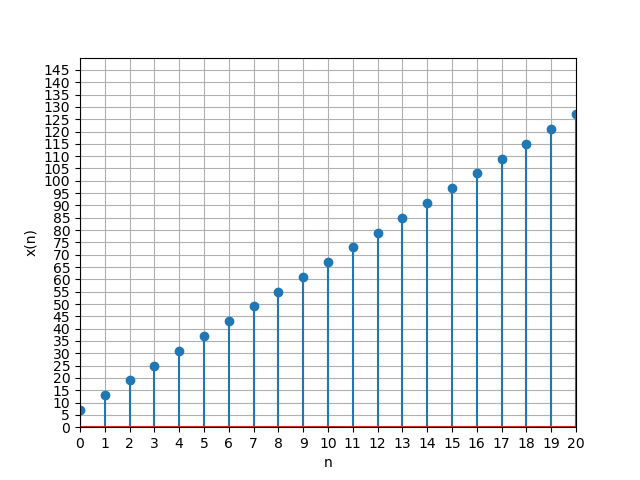
\includegraphics[width = 8cm]{Figure_1}\\
    Fig. 0. Plot of x\brak{n} \\
    \end{center}
\end{figure}
\begin{align}\label{eq:eq10}
   \lvert X\brak{z}\rvert = \sum_{n = -\infty}^{\infty}\lvert x\brak{n}z^{-n}\rvert < \infty
\end{align}

By equation \eqref{eq:eq4} :\\
For an infinite GP with ratio $z^{-1}$ to converge, we must have $|z^{-1}|< 1$ 
.Hence, for $X_{1}\brak{z}$ to converge, we must have  $|z^{-1}| < 1$ or $|z| > 1$.
\vspace{4mm}

\large\textbf{\brak{ii}} \normalsize The graph of $x_{2}$\brak{n} is :
\begin{figure}[!ht]
    \begin{center}
    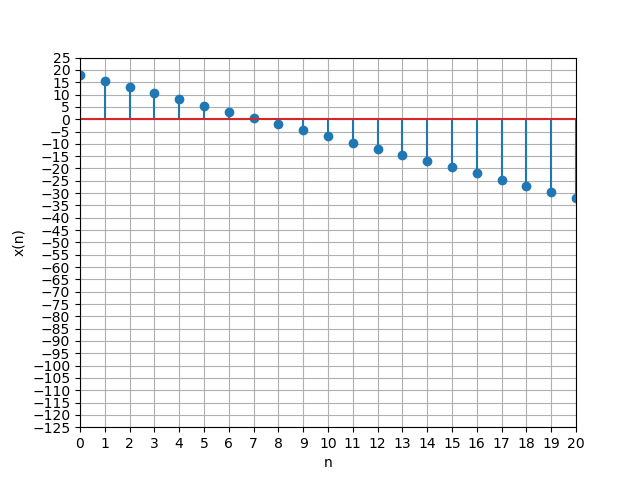
\includegraphics[width = 8cm]{Figure_2}\\
    Fig. 1. Plot of x\brak{n} \\
    \end{center}
\end{figure}

\FloatBarrier


By equation \eqref{eq:eq8} and \eqref{eq:eq10} :\\
For an infinite GP with ratio $z^{-1}$ to converge, we must have $|z^{-1}|< 1$ 
.Hence, for $X_{1}\brak{z}$ to converge, we must have  $|z^{-1}| < 1$ or $|z| > 1$.

\end{document}
